\documentclass[11pt]{report}
\usepackage[T1]{fontenc}
\usepackage{lmodern}
\usepackage{graphicx}
\usepackage{booktabs}
\usepackage{fancyhdr}
\usepackage[margin=1in,headheight=14pt]{geometry}

\pagestyle{fancy}
\fancyhf{}
\fancyhead[L]{\leftmark}
\fancyhead[R]{Test Report}
\fancyfoot[C]{Page \thepage}
\renewcommand{\headrulewidth}{0.4pt}
\renewcommand{\footrulewidth}{0.4pt}

\title{A Report on the Rendering of Documents}
\author{The Test Team}
\date{1 January 2026}

\begin{document}
\maketitle
\tableofcontents

\chapter{Introduction}\label{ch:intro}

This report tests the class report with the headers of fancyhdr, the
tables of booktabs, the lists, the footnotes, the cross-references, a
bibliography from BibTeX and figures in PNG, JPEG and PDF.\footnote{The
figures are in the folder of the report, beside the source.} The results
are in Chapter~\ref{ch:results}, and Table~\ref{tab:results} on
page~\pageref{tab:results} sums them up. The method follows
Knuth~\cite{knuth84} and Lamport~\cite{lamport94}.

\section{Lists}

A list can hold another list:
\begin{enumerate}
  \item The first step reads the file.
  \begin{itemize}
    \item It finds the class.
    \item It finds the packages.\footnote{A package that the tree does not
      hold is skipped.}
  \end{itemize}
  \item The second step sets the pages.
  \item The third step draws them.
\end{enumerate}
A description list names its items:
\begin{description}
  \item[Engine] The program that expands the macros.
  \item[Driver] The program that draws the boxes.
\end{description}

\chapter{Results}\label{ch:results}

\section{Tables}

Table~\ref{tab:results} uses the rules of booktabs and cells that span
columns.

\begin{table}[ht]
  \centering
  \caption{The results of three runs}\label{tab:results}
  \begin{tabular}{lrrr}
    \toprule
    & \multicolumn{2}{c}{Time (s)} & \\
    \cmidrule(lr){2-3}
    Document & First & Second & Pages \\
    \midrule
    Article & 0.21 & 0.18 & 3 \\
    Report  & 0.44 & 0.39 & 7 \\
    Book    & 1.02 & 0.95 & 24 \\
    \midrule
    \multicolumn{3}{l}{Total} & 34 \\
    \bottomrule
  \end{tabular}
\end{table}

\section{Figures}

Figure~\ref{fig:png} is a PNG image, Figure~\ref{fig:jpeg} a JPEG image and
Figure~\ref{fig:pdf} a PDF figure.

\begin{figure}[ht]
  \centering
  
\includegraphics[width=0.4\textwidth]{figures/shapes.png}
  \caption{An image in PNG}\label{fig:png}
\end{figure}

\begin{figure}[ht]
  \centering
  
\includegraphics[height=4cm]{figures/plasma.jpg}
  \caption{An image in JPEG}\label{fig:jpeg}
\end{figure}

\begin{figure}[ht]
  \centering
  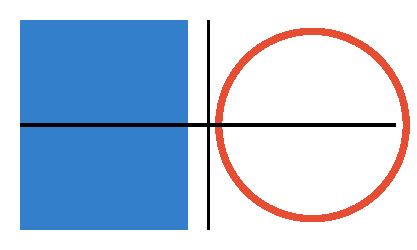
\includegraphics[width=5cm]{figures/vector}
  \caption{A figure in PDF}\label{fig:pdf}
\end{figure}

\section{Transforms}

The package graphicx turns, scales and reflects a box:
\rotatebox{30}{turned}, \scalebox{2}{large}, \scalebox{0.5}{small},
\reflectbox{mirror} and \resizebox{3cm}{!}{three centimeters}. It also
turns an image:

\begin{center}
  
\includegraphics[width=2cm,angle=90]{figures/shapes.png}
  \quad
  
\includegraphics[width=2cm,angle=-45]{figures/plasma.jpg}
\end{center}

\chapter{Conclusion}

Chapter~\ref{ch:intro} gave the method, and Chapter~\ref{ch:results}
gave the results~\cite{goossens94}.

\bibliographystyle{plain}
\bibliography{report}

\end{document}
